


% Header, overrides base

    % Make sure that the sphinx doc style knows who it inherits from.
    \def\sphinxdocclass{article}

    % Declare the document class
    \documentclass[letterpaper,10pt,english]{/usr/share/sphinx/texinputs/sphinxhowto}

    % Imports
    \usepackage[utf8]{inputenc}
    \DeclareUnicodeCharacter{00A0}{\\nobreakspace}
    \usepackage[T1]{fontenc}
    \usepackage{babel}
    \usepackage{times}
    \usepackage{import}
    \usepackage[Bjarne]{/usr/share/sphinx/texinputs/fncychap}
    \usepackage{longtable}
    \usepackage{/usr/share/sphinx/texinputs/sphinx}
    \usepackage{multirow}

    \usepackage{amsmath}
    \usepackage{amssymb}
    \usepackage{ucs}
    \usepackage{enumerate}

    % Used to make the Input/Output rules follow around the contents.
    \usepackage{needspace}

    % Pygments requirements
    \usepackage{fancyvrb}
    \usepackage{color}
    % ansi colors additions
    \definecolor{darkgreen}{rgb}{.12,.54,.11}
    \definecolor{lightgray}{gray}{.95}
    \definecolor{brown}{rgb}{0.54,0.27,0.07}
    \definecolor{purple}{rgb}{0.5,0.0,0.5}
    \definecolor{darkgray}{gray}{0.25}
    \definecolor{lightred}{rgb}{1.0,0.39,0.28}
    \definecolor{lightgreen}{rgb}{0.48,0.99,0.0}
    \definecolor{lightblue}{rgb}{0.53,0.81,0.92}
    \definecolor{lightpurple}{rgb}{0.87,0.63,0.87}
    \definecolor{lightcyan}{rgb}{0.5,1.0,0.83}

    % Needed to box output/input
    \usepackage{tikz}
        \usetikzlibrary{calc,arrows,shadows}
    \usepackage[framemethod=tikz]{mdframed}

    \usepackage{alltt}

    % Used to load and display graphics
    \usepackage{graphicx}
    \graphicspath{ {figs/} }
    \usepackage[Export]{adjustbox} % To resize

    % used so that images for notebooks which have spaces in the name can still be included
    \usepackage{grffile}


    % For formatting output while also word wrapping.
    \usepackage{listings}
    \lstset{breaklines=true}
    \lstset{basicstyle=\small\ttfamily}
    \def\smaller{\fontsize{9.5pt}{9.5pt}\selectfont}

    %Pygments definitions
    
\makeatletter
\def\PY@reset{\let\PY@it=\relax \let\PY@bf=\relax%
    \let\PY@ul=\relax \let\PY@tc=\relax%
    \let\PY@bc=\relax \let\PY@ff=\relax}
\def\PY@tok#1{\csname PY@tok@#1\endcsname}
\def\PY@toks#1+{\ifx\relax#1\empty\else%
    \PY@tok{#1}\expandafter\PY@toks\fi}
\def\PY@do#1{\PY@bc{\PY@tc{\PY@ul{%
    \PY@it{\PY@bf{\PY@ff{#1}}}}}}}
\def\PY#1#2{\PY@reset\PY@toks#1+\relax+\PY@do{#2}}

\expandafter\def\csname PY@tok@gd\endcsname{\def\PY@tc##1{\textcolor[rgb]{0.63,0.00,0.00}{##1}}}
\expandafter\def\csname PY@tok@gu\endcsname{\let\PY@bf=\textbf\def\PY@tc##1{\textcolor[rgb]{0.50,0.00,0.50}{##1}}}
\expandafter\def\csname PY@tok@gt\endcsname{\def\PY@tc##1{\textcolor[rgb]{0.00,0.27,0.87}{##1}}}
\expandafter\def\csname PY@tok@gs\endcsname{\let\PY@bf=\textbf}
\expandafter\def\csname PY@tok@gr\endcsname{\def\PY@tc##1{\textcolor[rgb]{1.00,0.00,0.00}{##1}}}
\expandafter\def\csname PY@tok@cm\endcsname{\let\PY@it=\textit\def\PY@tc##1{\textcolor[rgb]{0.25,0.50,0.50}{##1}}}
\expandafter\def\csname PY@tok@vg\endcsname{\def\PY@tc##1{\textcolor[rgb]{0.10,0.09,0.49}{##1}}}
\expandafter\def\csname PY@tok@m\endcsname{\def\PY@tc##1{\textcolor[rgb]{0.40,0.40,0.40}{##1}}}
\expandafter\def\csname PY@tok@mh\endcsname{\def\PY@tc##1{\textcolor[rgb]{0.40,0.40,0.40}{##1}}}
\expandafter\def\csname PY@tok@go\endcsname{\def\PY@tc##1{\textcolor[rgb]{0.53,0.53,0.53}{##1}}}
\expandafter\def\csname PY@tok@ge\endcsname{\let\PY@it=\textit}
\expandafter\def\csname PY@tok@vc\endcsname{\def\PY@tc##1{\textcolor[rgb]{0.10,0.09,0.49}{##1}}}
\expandafter\def\csname PY@tok@il\endcsname{\def\PY@tc##1{\textcolor[rgb]{0.40,0.40,0.40}{##1}}}
\expandafter\def\csname PY@tok@cs\endcsname{\let\PY@it=\textit\def\PY@tc##1{\textcolor[rgb]{0.25,0.50,0.50}{##1}}}
\expandafter\def\csname PY@tok@cp\endcsname{\def\PY@tc##1{\textcolor[rgb]{0.74,0.48,0.00}{##1}}}
\expandafter\def\csname PY@tok@gi\endcsname{\def\PY@tc##1{\textcolor[rgb]{0.00,0.63,0.00}{##1}}}
\expandafter\def\csname PY@tok@gh\endcsname{\let\PY@bf=\textbf\def\PY@tc##1{\textcolor[rgb]{0.00,0.00,0.50}{##1}}}
\expandafter\def\csname PY@tok@ni\endcsname{\let\PY@bf=\textbf\def\PY@tc##1{\textcolor[rgb]{0.60,0.60,0.60}{##1}}}
\expandafter\def\csname PY@tok@nl\endcsname{\def\PY@tc##1{\textcolor[rgb]{0.63,0.63,0.00}{##1}}}
\expandafter\def\csname PY@tok@nn\endcsname{\let\PY@bf=\textbf\def\PY@tc##1{\textcolor[rgb]{0.00,0.00,1.00}{##1}}}
\expandafter\def\csname PY@tok@no\endcsname{\def\PY@tc##1{\textcolor[rgb]{0.53,0.00,0.00}{##1}}}
\expandafter\def\csname PY@tok@na\endcsname{\def\PY@tc##1{\textcolor[rgb]{0.49,0.56,0.16}{##1}}}
\expandafter\def\csname PY@tok@nb\endcsname{\def\PY@tc##1{\textcolor[rgb]{0.00,0.50,0.00}{##1}}}
\expandafter\def\csname PY@tok@nc\endcsname{\let\PY@bf=\textbf\def\PY@tc##1{\textcolor[rgb]{0.00,0.00,1.00}{##1}}}
\expandafter\def\csname PY@tok@nd\endcsname{\def\PY@tc##1{\textcolor[rgb]{0.67,0.13,1.00}{##1}}}
\expandafter\def\csname PY@tok@ne\endcsname{\let\PY@bf=\textbf\def\PY@tc##1{\textcolor[rgb]{0.82,0.25,0.23}{##1}}}
\expandafter\def\csname PY@tok@nf\endcsname{\def\PY@tc##1{\textcolor[rgb]{0.00,0.00,1.00}{##1}}}
\expandafter\def\csname PY@tok@si\endcsname{\let\PY@bf=\textbf\def\PY@tc##1{\textcolor[rgb]{0.73,0.40,0.53}{##1}}}
\expandafter\def\csname PY@tok@s2\endcsname{\def\PY@tc##1{\textcolor[rgb]{0.73,0.13,0.13}{##1}}}
\expandafter\def\csname PY@tok@vi\endcsname{\def\PY@tc##1{\textcolor[rgb]{0.10,0.09,0.49}{##1}}}
\expandafter\def\csname PY@tok@nt\endcsname{\let\PY@bf=\textbf\def\PY@tc##1{\textcolor[rgb]{0.00,0.50,0.00}{##1}}}
\expandafter\def\csname PY@tok@nv\endcsname{\def\PY@tc##1{\textcolor[rgb]{0.10,0.09,0.49}{##1}}}
\expandafter\def\csname PY@tok@s1\endcsname{\def\PY@tc##1{\textcolor[rgb]{0.73,0.13,0.13}{##1}}}
\expandafter\def\csname PY@tok@sh\endcsname{\def\PY@tc##1{\textcolor[rgb]{0.73,0.13,0.13}{##1}}}
\expandafter\def\csname PY@tok@sc\endcsname{\def\PY@tc##1{\textcolor[rgb]{0.73,0.13,0.13}{##1}}}
\expandafter\def\csname PY@tok@sx\endcsname{\def\PY@tc##1{\textcolor[rgb]{0.00,0.50,0.00}{##1}}}
\expandafter\def\csname PY@tok@bp\endcsname{\def\PY@tc##1{\textcolor[rgb]{0.00,0.50,0.00}{##1}}}
\expandafter\def\csname PY@tok@c1\endcsname{\let\PY@it=\textit\def\PY@tc##1{\textcolor[rgb]{0.25,0.50,0.50}{##1}}}
\expandafter\def\csname PY@tok@kc\endcsname{\let\PY@bf=\textbf\def\PY@tc##1{\textcolor[rgb]{0.00,0.50,0.00}{##1}}}
\expandafter\def\csname PY@tok@c\endcsname{\let\PY@it=\textit\def\PY@tc##1{\textcolor[rgb]{0.25,0.50,0.50}{##1}}}
\expandafter\def\csname PY@tok@mf\endcsname{\def\PY@tc##1{\textcolor[rgb]{0.40,0.40,0.40}{##1}}}
\expandafter\def\csname PY@tok@err\endcsname{\def\PY@bc##1{\setlength{\fboxsep}{0pt}\fcolorbox[rgb]{1.00,0.00,0.00}{1,1,1}{\strut ##1}}}
\expandafter\def\csname PY@tok@kd\endcsname{\let\PY@bf=\textbf\def\PY@tc##1{\textcolor[rgb]{0.00,0.50,0.00}{##1}}}
\expandafter\def\csname PY@tok@ss\endcsname{\def\PY@tc##1{\textcolor[rgb]{0.10,0.09,0.49}{##1}}}
\expandafter\def\csname PY@tok@sr\endcsname{\def\PY@tc##1{\textcolor[rgb]{0.73,0.40,0.53}{##1}}}
\expandafter\def\csname PY@tok@mo\endcsname{\def\PY@tc##1{\textcolor[rgb]{0.40,0.40,0.40}{##1}}}
\expandafter\def\csname PY@tok@kn\endcsname{\let\PY@bf=\textbf\def\PY@tc##1{\textcolor[rgb]{0.00,0.50,0.00}{##1}}}
\expandafter\def\csname PY@tok@mi\endcsname{\def\PY@tc##1{\textcolor[rgb]{0.40,0.40,0.40}{##1}}}
\expandafter\def\csname PY@tok@gp\endcsname{\let\PY@bf=\textbf\def\PY@tc##1{\textcolor[rgb]{0.00,0.00,0.50}{##1}}}
\expandafter\def\csname PY@tok@o\endcsname{\def\PY@tc##1{\textcolor[rgb]{0.40,0.40,0.40}{##1}}}
\expandafter\def\csname PY@tok@kr\endcsname{\let\PY@bf=\textbf\def\PY@tc##1{\textcolor[rgb]{0.00,0.50,0.00}{##1}}}
\expandafter\def\csname PY@tok@s\endcsname{\def\PY@tc##1{\textcolor[rgb]{0.73,0.13,0.13}{##1}}}
\expandafter\def\csname PY@tok@kp\endcsname{\def\PY@tc##1{\textcolor[rgb]{0.00,0.50,0.00}{##1}}}
\expandafter\def\csname PY@tok@w\endcsname{\def\PY@tc##1{\textcolor[rgb]{0.73,0.73,0.73}{##1}}}
\expandafter\def\csname PY@tok@kt\endcsname{\def\PY@tc##1{\textcolor[rgb]{0.69,0.00,0.25}{##1}}}
\expandafter\def\csname PY@tok@ow\endcsname{\let\PY@bf=\textbf\def\PY@tc##1{\textcolor[rgb]{0.67,0.13,1.00}{##1}}}
\expandafter\def\csname PY@tok@sb\endcsname{\def\PY@tc##1{\textcolor[rgb]{0.73,0.13,0.13}{##1}}}
\expandafter\def\csname PY@tok@k\endcsname{\let\PY@bf=\textbf\def\PY@tc##1{\textcolor[rgb]{0.00,0.50,0.00}{##1}}}
\expandafter\def\csname PY@tok@se\endcsname{\let\PY@bf=\textbf\def\PY@tc##1{\textcolor[rgb]{0.73,0.40,0.13}{##1}}}
\expandafter\def\csname PY@tok@sd\endcsname{\let\PY@it=\textit\def\PY@tc##1{\textcolor[rgb]{0.73,0.13,0.13}{##1}}}

\def\PYZbs{\char`\\}
\def\PYZus{\char`\_}
\def\PYZob{\char`\{}
\def\PYZcb{\char`\}}
\def\PYZca{\char`\^}
\def\PYZam{\char`\&}
\def\PYZlt{\char`\<}
\def\PYZgt{\char`\>}
\def\PYZsh{\char`\#}
\def\PYZpc{\char`\%}
\def\PYZdl{\char`\$}
\def\PYZhy{\char`\-}
\def\PYZsq{\char`\'}
\def\PYZdq{\char`\"}
\def\PYZti{\char`\~}
% for compatibility with earlier versions
\def\PYZat{@}
\def\PYZlb{[}
\def\PYZrb{]}
\makeatother


    %Set pygments styles if needed...
    
        \definecolor{nbframe-border}{rgb}{0.867,0.867,0.867}
        \definecolor{nbframe-bg}{rgb}{0.969,0.969,0.969}
        \definecolor{nbframe-in-prompt}{rgb}{0.0,0.0,0.502}
        \definecolor{nbframe-out-prompt}{rgb}{0.545,0.0,0.0}

        \newenvironment{ColorVerbatim}
        {\begin{mdframed}[%
            roundcorner=1.0pt, %
            backgroundcolor=nbframe-bg, %
            userdefinedwidth=1\linewidth, %
            leftmargin=0.1\linewidth, %
            innerleftmargin=0pt, %
            innerrightmargin=0pt, %
            linecolor=nbframe-border, %
            linewidth=1pt, %
            usetwoside=false, %
            everyline=true, %
            innerlinewidth=3pt, %
            innerlinecolor=nbframe-bg, %
            middlelinewidth=1pt, %
            middlelinecolor=nbframe-bg, %
            outerlinewidth=0.5pt, %
            outerlinecolor=nbframe-border, %
            needspace=0pt
        ]}
        {\end{mdframed}}
        
        \newenvironment{InvisibleVerbatim}
        {\begin{mdframed}[leftmargin=0.1\linewidth,innerleftmargin=3pt,innerrightmargin=3pt, userdefinedwidth=1\linewidth, linewidth=0pt, linecolor=white, usetwoside=false]}
        {\end{mdframed}}

        \renewenvironment{Verbatim}[1][\unskip]
        {\begin{alltt}\smaller}
        {\end{alltt}}
    

    % Help prevent overflowing lines due to urls and other hard-to-break 
    % entities.  This doesn't catch everything...
    \sloppy

    % Document level variables
    \title{Computational Methods in Biology}
    \date{January 26, 2015}
    \release{}
    \author{Nathan Crock}
    \renewcommand{\releasename}{}

    % TODO: Add option for the user to specify a logo for his/her export.
    \newcommand{\sphinxlogo}{}

    % Make the index page of the document.
    \makeindex

    % Import sphinx document type specifics.
     


% Body

    % Start of the document
    \begin{document}

        
            \maketitle
        

        


        
\section{Assignment 1}\label{computational-methods-in-biology---assignment-1}

\subsection{Probelm 1.}\label{probelm-1.}

\subsubsection{(a)}\label{a}

The Nernst Potential is given by:

\[V_S = \frac{RT}{zF}\ln\bigg(\frac{[S]_o}{[S]_i}\bigg)\]

Where $R=8.314$ is the gas constant, $T$ is the temperature in Kelvin,
$z$ is the valence charge of the ion, and $F=9.648\times10^4$ is
Faraday's constant. For simplicity, I will write a \emph{nernst}
function to calculate the potentials for an ion based on its
intracellular and extracellular concentrations, its valence charge z,
and the temperature of their solution in Celcius.

    % Make sure that atleast 4 lines are below the HR
    \needspace{4\baselineskip}

    
        \vspace{6pt}
        \makebox[0.1\linewidth]{\smaller\hfill\tt\color{nbframe-in-prompt}In\hspace{4pt}{[}6{]}:\hspace{4pt}}\\*
        \vspace{-2.65\baselineskip}
        \begin{ColorVerbatim}
            \vspace{-0.7\baselineskip}
            \begin{Verbatim}[commandchars=\\\{\}]
\PY{k+kn}{import} \PY{n+nn}{numpy} \PY{k+kn}{as} \PY{n+nn}{np}  \PY{c}{\PYZsh{} Use the numerics library for math}

\PY{k}{def} \PY{n+nf}{nernst}\PY{p}{(}\PY{n}{intra}\PY{p}{,} \PY{n}{extra}\PY{p}{,} \PY{n}{C}\PY{p}{,} \PY{n}{z}\PY{p}{)}\PY{p}{:}
    \PY{n}{R} \PY{o}{=} \PY{l+m+mf}{8.314462}  \PY{c}{\PYZsh{} Gas Constant}
    \PY{n}{F} \PY{o}{=} \PY{l+m+mf}{9.64853399e4}  \PY{c}{\PYZsh{} Faraday\PYZsq{}s Constant}
    \PY{n}{T} \PY{o}{=} \PY{l+m+mf}{273.15} \PY{o}{+} \PY{n}{C}  \PY{c}{\PYZsh{} Kelvin = 273.15 + Celcius}
    
    \PY{k}{return} \PY{p}{(}\PY{n}{R}\PY{o}{*}\PY{n}{T}\PY{p}{)}\PY{o}{/}\PY{p}{(}\PY{n}{z}\PY{o}{*}\PY{n}{F}\PY{p}{)}\PY{o}{*}\PY{p}{(}\PY{n}{np}\PY{o}{.}\PY{n}{log}\PY{p}{(}\PY{n+nb}{float}\PY{p}{(}\PY{n}{extra}\PY{p}{)}\PY{o}{/}\PY{n}{intra}\PY{p}{)}\PY{p}{)}
\end{Verbatim}

            
                \vspace{-0.2\baselineskip}
            
        \end{ColorVerbatim}
    
For Potassium we are given $[K]_i=430$ and $[K]_o=20$. The temperature
is $20^o$ Celcius and Potassium has a valence charge of $+1$.
Therefore\ldots{}


    \hspace{1pt}
    % Make sure that atleast 4 lines are below the HR
    \needspace{4\baselineskip}

    
        \vspace{6pt}
        \makebox[0.1\linewidth]{\smaller\hfill\tt\color{nbframe-in-prompt}In\hspace{4pt}{[}7{]}:\hspace{4pt}}\\*
        \vspace{-2.65\baselineskip}
        \begin{ColorVerbatim}
            \vspace{-0.7\baselineskip}
            \begin{Verbatim}[commandchars=\\\{\}]
\PY{n}{intra} \PY{o}{=} \PY{l+m+mi}{430}
\PY{n}{extra} \PY{o}{=} \PY{l+m+mi}{20}
\PY{n}{C} \PY{o}{=} \PY{l+m+mi}{20}
\PY{n}{z} \PY{o}{=} \PY{l+m+mi}{1}

\PY{n}{Vk} \PY{o}{=} \PY{n}{nernst}\PY{p}{(}\PY{n}{intra}\PY{p}{,}\PY{n}{extra}\PY{p}{,}\PY{n}{C}\PY{p}{,}\PY{n}{z}\PY{p}{)}\PY{p}{;} \PY{n}{Vk}
\end{Verbatim}

            
                \vspace{-0.2\baselineskip}
            
        \end{ColorVerbatim}
    

    

        % If the first block is an image, minipage the image.  Else
        % request a certain amount of space for the input text.
        \needspace{4\baselineskip}
        
        

            % Add document contents.
            
                \makebox[0.1\linewidth]{\smaller\hfill\tt\color{nbframe-out-prompt}Out\hspace{4pt}{[}7{]}:\hspace{4pt}}\\*
                \vspace{-2.55\baselineskip}\begin{InvisibleVerbatim}
                \vspace{-0.5\baselineskip}
                \hspace{1pt}

\begin{alltt}-0.077504259044191351\end{alltt}

            \end{InvisibleVerbatim}
            
        
    
Which is approximately $-77.5$ mVFor Sodium we are given $[Na]_i=50$ and $[Na]_o=440$. The temperature is
$20^o$ Celcius and Sodium has a valence charge of $+1$.
Therefore\ldots{}


    \hspace{1pt}
    % Make sure that atleast 4 lines are below the HR
    \needspace{4\baselineskip}

    
        \vspace{6pt}
        \makebox[0.1\linewidth]{\smaller\hfill\tt\color{nbframe-in-prompt}In\hspace{4pt}{[}8{]}:\hspace{4pt}}\\*
        \vspace{-2.65\baselineskip}
        \begin{ColorVerbatim}
            \vspace{-0.7\baselineskip}
            \begin{Verbatim}[commandchars=\\\{\}]
\PY{n}{intra} \PY{o}{=} \PY{l+m+mi}{50}
\PY{n}{extra} \PY{o}{=} \PY{l+m+mi}{440}
\PY{n}{C} \PY{o}{=} \PY{l+m+mi}{20}
\PY{n}{z} \PY{o}{=} \PY{l+m+mi}{1}

\PY{n}{Vna} \PY{o}{=} \PY{n}{nernst}\PY{p}{(}\PY{n}{intra}\PY{p}{,}\PY{n}{extra}\PY{p}{,}\PY{n}{C}\PY{p}{,}\PY{n}{z}\PY{p}{)}\PY{p}{;} \PY{n}{Vna}
\end{Verbatim}

            
                \vspace{-0.2\baselineskip}
            
        \end{ColorVerbatim}
    

    

        % If the first block is an image, minipage the image.  Else
        % request a certain amount of space for the input text.
        \needspace{4\baselineskip}
        
        

            % Add document contents.
            
                \makebox[0.1\linewidth]{\smaller\hfill\tt\color{nbframe-out-prompt}Out\hspace{4pt}{[}8{]}:\hspace{4pt}}\\*
                \vspace{-2.55\baselineskip}\begin{InvisibleVerbatim}
                \vspace{-0.5\baselineskip}
                \hspace{1pt}

\begin{alltt}0.054937944143186326\end{alltt}

            \end{InvisibleVerbatim}
            
        
    
Which is approximately $54.9$ mVFor Chloride we are given $[Cl]_i=65$ and $[Cl]_o=560$. The temperature
is $20^o$ Celcius and Chloride has a valence charge of $-1$.
Therefore\ldots{}


    \hspace{1pt}
    % Make sure that atleast 4 lines are below the HR
    \needspace{4\baselineskip}

    
        \vspace{6pt}
        \makebox[0.1\linewidth]{\smaller\hfill\tt\color{nbframe-in-prompt}In\hspace{4pt}{[}9{]}:\hspace{4pt}}\\*
        \vspace{-2.65\baselineskip}
        \begin{ColorVerbatim}
            \vspace{-0.7\baselineskip}
            \begin{Verbatim}[commandchars=\\\{\}]
\PY{n}{intra} \PY{o}{=} \PY{l+m+mi}{65}
\PY{n}{extra} \PY{o}{=} \PY{l+m+mi}{560}
\PY{n}{C} \PY{o}{=} \PY{l+m+mi}{20}
\PY{n}{z} \PY{o}{=} \PY{o}{\PYZhy{}}\PY{l+m+mi}{1}

\PY{n}{Vcl} \PY{o}{=} \PY{n}{nernst}\PY{p}{(}\PY{n}{intra}\PY{p}{,}\PY{n}{extra}\PY{p}{,}\PY{n}{C}\PY{p}{,}\PY{n}{z}\PY{p}{)}\PY{p}{;} \PY{n}{Vcl}
\end{Verbatim}

            
                \vspace{-0.2\baselineskip}
            
        \end{ColorVerbatim}
    

    

        % If the first block is an image, minipage the image.  Else
        % request a certain amount of space for the input text.
        \needspace{4\baselineskip}
        
        

            % Add document contents.
            
                \makebox[0.1\linewidth]{\smaller\hfill\tt\color{nbframe-out-prompt}Out\hspace{4pt}{[}9{]}:\hspace{4pt}}\\*
                \vspace{-2.55\baselineskip}\begin{InvisibleVerbatim}
                \vspace{-0.5\baselineskip}
                \hspace{1pt}

\begin{alltt}-0.054402340153032386\end{alltt}

            \end{InvisibleVerbatim}
            
        
    
Which is approximately $-54.4$ mV\subsubsection{(b)}\label{b}

The resting membrane potential is given by the weighted average of
Nernst Potentials

\[ V_{rest} = \frac{g_KV_K + g_{Na}V_{Na} + g_{Cl}V_{Cl}}{g_K + g_{Na} + g_{Cl}} \]

Given $g_{Na} = 1$, $g_K = 10$, $g_{Cl} = 3$, and the Nernst Potentials
found above we can calculate the resting potential\ldots{}

    \hspace{1pt}
    % Make sure that atleast 4 lines are below the HR
    \needspace{4\baselineskip}

    
        \vspace{6pt}
        \makebox[0.1\linewidth]{\smaller\hfill\tt\color{nbframe-in-prompt}In\hspace{4pt}{[}10{]}:\hspace{4pt}}\\*
        \vspace{-2.65\baselineskip}
        \begin{ColorVerbatim}
            \vspace{-0.7\baselineskip}
            \begin{Verbatim}[commandchars=\\\{\}]
\PY{n}{gna} \PY{o}{=} \PY{l+m+mi}{1}
\PY{n}{gk} \PY{o}{=} \PY{l+m+mi}{10}
\PY{n}{gcl} \PY{o}{=} \PY{l+m+mi}{3}

\PY{n}{Vrest} \PY{o}{=} \PY{p}{(}\PY{n}{gk}\PY{o}{*}\PY{n}{Vk} \PY{o}{+} \PY{n}{gna}\PY{o}{*}\PY{n}{Vna} \PY{o}{+} \PY{n}{gcl}\PY{o}{*}\PY{n}{Vcl}\PY{p}{)} \PY{o}{/} \PY{p}{(}\PY{n}{gk} \PY{o}{+} \PY{n}{gna} \PY{o}{+} \PY{n}{gcl}\PY{p}{)}\PY{p}{;} \PY{n}{Vrest}
\end{Verbatim}

            
                \vspace{-0.2\baselineskip}
            
        \end{ColorVerbatim}
    

    

        % If the first block is an image, minipage the image.  Else
        % request a certain amount of space for the input text.
        \needspace{4\baselineskip}
        
        

            % Add document contents.
            
                \makebox[0.1\linewidth]{\smaller\hfill\tt\color{nbframe-out-prompt}Out\hspace{4pt}{[}10{]}:\hspace{4pt}}\\*
                \vspace{-2.55\baselineskip}\begin{InvisibleVerbatim}
                \vspace{-0.5\baselineskip}
                \hspace{1pt}

\begin{alltt}-0.063093690482701734\end{alltt}

            \end{InvisibleVerbatim}
            
        
    
Which is approximately -63.1 mV\subsection{Problem 2}\label{problem-2}

\subsubsection{(a)}\label{a}

We will solve the passive membrane equation

\[C\frac{dV}{dt}=-g(V-V_{rev})+I_{app}\]

using the integrating factor technique. First let us divide the equation
through by C and rewrite it as follows\ldots{}

\[\frac{dV}{dt}+\frac{1}{\tau}V=Q\]

where we used the fact that the conductance $g=\frac{1}{R}$ and the
membrane time constant $\tau=RC$ and to simplify algebra we let

\[\frac{1}{\tau}V_{rev}+\frac{1}{C}I_{app}=Q\]

We now have the linear ODE in standard form and by letting
$\frac{dV}{dt}=0$ we can easily see the steady state of the system
$V_{\infty}= \tau Q$. Now we apply the integrating factor technique.
Multiply both sides through by exp($\int_0^t\frac{1}{\tau}dt$) =
$e^{\frac{t}{\tau}}$.

\[e^{\frac{t}{\tau}}\Big(\frac{dV}{dt}+\frac{1}{\tau}V\Big)=e^{\frac{t}{\tau}}Q\]

After distributing the exponential on the left side it can be rewritten
as a product rule

\[e^{\frac{t}{\tau}}\frac{dV}{dt}+\frac{1}{\tau}e^{\frac{t}{\tau}}V \Rightarrow \frac{d}{dt}(e^{\frac{t}{\tau}}V)\]

No if we integrate both sides\ldots{}

\[\int_0^t \frac{d}{ds}(e^{\frac{s}{\tau}}V) ds = Q \int_0^t e^{\frac{s}{\tau}}ds\]

\[e^{\frac{t}{\tau}}V(t)-V_0 = \tau Q (e^{\frac{t}{\tau}}-1)\]

\[V(t)= e^{-\frac{t}{\tau}}V_0+\tau Q(1-e^{-\frac{t}{\tau}})\]

The solution confirms the behavior we would expect. At $t=0$ we see that
$V(t)=V_0$. Now as time passes, exp($-\frac{t}{\tau}$) $\rightarrow 0$
which slowly shifts $V(t)$ from the first term $V_0$ (the initial
condition) to the second term $\tau Q$ which we already established was
the system's steady state. So with a substitution $\tau Q=V_{\infty}$
and some simple algebra we can rewrite our solution as

\[V(t) = (V_0-V_{\infty})e^{-\frac{t}{\tau}}+V_{\infty}\]

\subsubsection{(b)}\label{b}

The $\tau$ parameter is the time constant for the differential equation.
It controls the speed of the approach to steady state. It is the product
of both the resistance and capacitance of the membrane $\tau=RC$. If one
wanted to vary the growth/decay rate of the voltage they could do so by
changing the resistance or the capacitance.\subsection{Problem 3}\label{problem-3}

Given the Nernst-Planck equation

\[J = -D\Big(\frac{dC}{dx}+\frac{zCF}{RT}\frac{d\Phi}{dx}\Big)\]

we can derive the Nerst equation by finding the potential when flux is
zero. We set $J=0$ and divide through by $-D$

\[0=\frac{dC}{dx}+\frac{zCF}{RT}\frac{d\Phi}{dx}\]

To put this into more of an integral friendly form we will isolate the
$\frac{d\Phi}{dx}$ term and group the concentration variable $C$.

\[\frac{d\Phi}{dx}=-\frac{RT}{zF}\frac{\frac{dC}{dx}}{C}\]

Next we integrate through\ldots{}

\[\int_0^x \frac{d\Phi}{ds} ds = -\frac{RT}{zF} \int_0^x \frac{\frac{dC}{ds}}{C} ds \hspace{10pt} \Rightarrow \hspace{10pt} \Phi(x)-\Phi(0) = -\frac{RT}{zF}(\ln(C(x))-\ln(C(0)))\]

Where is $x=0$? The convention is to define $x=0$ to be extracellular.
Also, because voltage is defined as the potential of a charge relative
to some source of electric field and the source is not explicitly
defined here, we can define $\Phi(0)=0$. The source is irrelevant, we
are only interested in the difference of potentials across the membrane.
Therefore $\Phi(x)-\Phi(0) = V$.

\[V = -\frac{RT}{zF}(\ln(C(x))-\ln(C(0)))\]

Lastly we use logarithmic properties to combine the natural logs. We
move the $-1$ to the exponent of the natural log flipping the inner
fraction, and redefine the concentrations $C(x)=[C_{in}]$ and
$C(0)=[C_{out}]$ giving us the Nernst equation\ldots{}

\[V = \frac{RT}{zF}\ln\Big(\frac{[C_{out}]}{[C_{in}]}\Big)\]\subsection{Problem 4}\label{problem-4}

\subsubsection{(a)}\label{a}

The driving force $V-V_{rev}$ is simply a translation of the voltage up
or down. Below we have the original voltage plot provided.

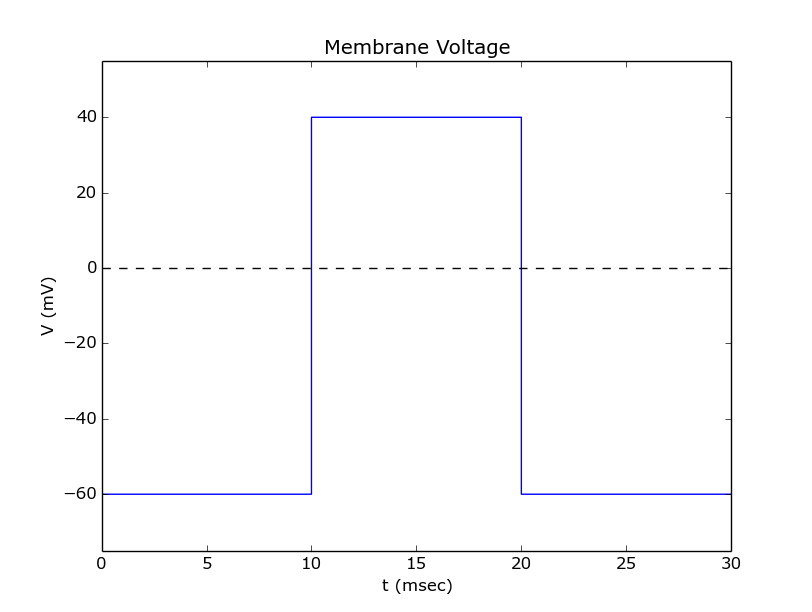
\includegraphics[scale=.5]{vRest.png}

Given $V_K = -70$mV the plot for $V-V_K$ is a vertical translation
upwards by $70$mV.

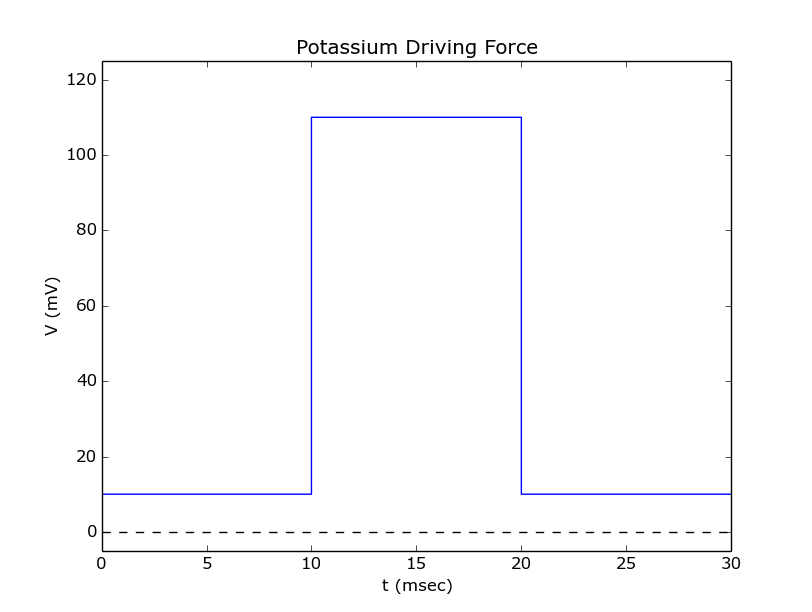
\includegraphics[scale=.5]{vKforce.png}

This simply means when the membrane voltage is at rest, $V=-60$mV, the
potassium reversal potential wants to drive the voltage down to $-70$mV
with a ``driving force'' of $10$mV. Similarly when the voltage jumps to
$V=40$mV the potassium reversal potential wants to drive the voltage way
down to $-70$mV with a much stronger ``driving force'' of $110$mV.

Given $V_{Na} = 50$mV the plot for $V-V_{Na}$ is a vertical translation
downwards by $50$mV. We interpret this plot the same as above.

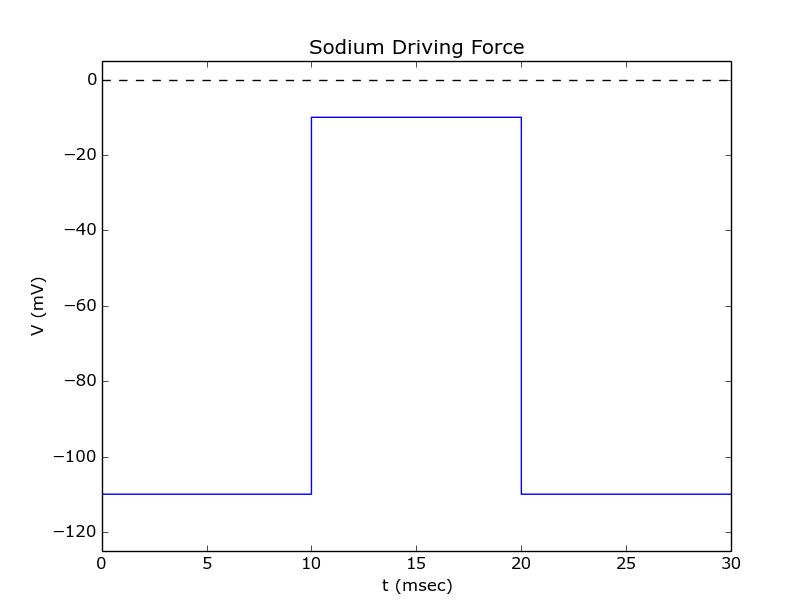
\includegraphics[scale=.5]{vNaforce.png}

\subsubsection{(b)}\label{b}

The three differential equations governing the probability of the ion
channels being opened or closed (activated or inactivated) are given by

\[\frac{dn}{dt} = \frac{n_{\infty}(V)-n}{\tau_n(V)} \hspace{25pt} \frac{dm}{dt} = \frac{m_{\infty}(V)-m}{\tau_m(V)} \hspace{25pt} \frac{dh}{dt} = \frac{h_{\infty}(V)-h}{\tau_h(V)}\]

We notice that each equation is a function of voltage and, as evidenced
by our initial voltage plot, voltage is held constant for t
$\epsilon (0,10)\bigcup (10,20) \bigcup (20,30)$. Therefore the steady
states and the (variable) time constants each become constant. This
means the nonlinear ODEs becomes linear on those intervals and we can
solve them analytically for piecewise solutions. Because all of the
equations have a similar form, we will solve a general expression giving
us the solution for all of the equations on all the intervals. Let $x$
be the particular gating variable, then

\[\frac{dx}{dt} = \frac{x_{\infty}(V)-x}{\tau_x(V)}\]

Now we allow our functions of voltage to become constants
$x_{\infty}(V)=x_{\infty}$ and $\tau_x(V)=\tau_x$

\[\frac{dx}{dt} = \frac{x_{\infty}-x}{\tau_x} \hspace{10pt} \Rightarrow \hspace{10pt} \frac{dx}{dt} +\frac{1}{\tau_x}x = Q\]

Where $Q = \frac{x_{\infty}}{\tau_x}$. This the same standard form used
in problem 2a. Using the same technique we arrive at the same solution.

\[x(t) = (x_0-x^*_{\infty})e^{-\frac{t}{\tau_x}}+x^*_{\infty}\]

Where
$x^*_{\infty} = \tau_xQ = \tau_x\big(\frac{x_{\infty}}{\tau_x}\big) = x_{\infty}$.
This gives us our general solution for all of the gating variables.

\[x(t) = (x_0-x_{\infty})e^{-\frac{t}{\tau_x}}+x_{\infty}\]

For each gating variable, the time constants were provided:
$\tau_m=0.5$msec, $\tau_n=5$msec and $\tau_h=5$msec. What remains to be
determined are the initial conditions and the steady states for each
gating variable. These will be crude approximations to the behavior
because to approximate the continuous behavior over the discontiuous
jumps we'll be using the final values of the previous interval as the
initial conditions for its neighboring interval. These change depending
on which interval we are solving over. We will start with t
$\epsilon [0,10)$. In these ranges, the voltage is at rest, so the
sodium and potassium activation gates are closed, and the sodium
inactivation gate is opened, $n_0=0$, $m_0=0$, $h_0=1$. Also, at
$-60$mV, the steady states for each gating variable is approximately,
$n_{\infty}=0$, $m_{\infty}=0$, $h_{\infty}=1$. Substituting these
values into each gating variable's equation gives us the following
expressions

\[n(t) = (n_0-n_{\infty})e^{-\frac{t}{\tau_n}}+n_{\infty} \hspace{23pt} \Rightarrow \hspace{10pt} n(t) = (0-0)e^{-\frac{t}{5}}+0 \hspace{10pt} = 0\]
\[m(t) = (m_0-m_{\infty})e^{-\frac{t}{\tau_m}}+m_{\infty} \hspace{10pt} \Rightarrow \hspace{10pt} m(t) = (0-0)e^{-\frac{t}{0.5}}+0 \hspace{4pt} = 0\]
\[h(t) = (h_0-h_{\infty})e^{-\frac{t}{\tau_h}}+h_{\infty} \hspace{24pt} \Rightarrow \hspace{10pt} h(t) = (1-1)e^{-\frac{t}{5}}+1 \hspace{11pt} = 1\]

Now we will determine the constants for t $\epsilon [10,20]$. We take
the values of the gating variable before the jump to be the initial
conditions in this interval. They are $n_0=0$, $m_0=0$, $h_0=1$. At
$40$mV, the steady states for each gating variable is approximately,
$n_{\infty}=1$, $m_{\infty}=1$, $h_{\infty}=0$. Substituting these
values into each gating variable's equation gives us the following
expressions

\[n(t) = (n_0-n_{\infty})e^{-\frac{t}{\tau_n}}+n_{\infty} \hspace{23pt} \Rightarrow \hspace{10pt} n(t) = (0-1)e^{-\frac{t}{5}}+1 \hspace{10pt} = 1-e^{-\frac{t}{5}}\]
\[m(t) = (m_0-m_{\infty})e^{-\frac{t}{\tau_m}}+m_{\infty} \hspace{10pt} \Rightarrow \hspace{10pt} m(t) = (0-1)e^{-\frac{t}{0.5}}+1 \hspace{4pt} = 1-e^{-\frac{t}{0.5}}\]
\[h(t) = (h_0-h_{\infty})e^{-\frac{t}{\tau_h}}+h_{\infty} \hspace{24pt} \Rightarrow \hspace{10pt} h(t) = (1-0)e^{-\frac{t}{5}}+0 \hspace{11pt} = e^{-\frac{t}{5}}\]

On the last interval, t $\epsilon (20,30]$, again the initial conditions
will come from the previous interval and the steady states will depend
on the voltage. The initial conditions are the previous interval's
gating variables evaluated at $t=10$. It is at $10$ because when solving
the differential equation over the middle interval, the ion channels are
just opening at $t=10$. So their behavior from $t=10$ to $t=20$ is what
the functions would do from $t=0$ to $t=10$. The initial conditions are,
$n_0=1-e^{-2}$, $m_0=1-e^{-20}$, $h_0=e^{-2}$. The steady states are the
same as the first interval, $n_{\infty}=0$, $m_{\infty}=0$,
$h_{\infty}=1$. Plugging these into our equations gives

\[n(t) = (n_0-n_{\infty})e^{-\frac{t}{\tau_n}}+n_{\infty} \hspace{23pt} \Rightarrow \hspace{10pt} n(t) = (1-e^{-4}-0)e^{-\frac{t}{5}}+0 \hspace{14pt} = (1-e^{-4})e^{-\frac{t}{5}}\]
\[m(t) = (m_0-m_{\infty})e^{-\frac{t}{\tau_m}}+m_{\infty} \hspace{10pt} \Rightarrow \hspace{10pt} m(t) = (1-e^{-40}-0)e^{-\frac{t}{0.5}}+0 \hspace{4pt} = (1-e^{-40})e^{-\frac{t}{0.5}}\]
\[h(t) = (h_0-h_{\infty})e^{-\frac{t}{\tau_h}}+h_{\infty} \hspace{24pt} \Rightarrow \hspace{10pt} h(t) = (e^{-4}-1)e^{-\frac{t}{5}}+1 \hspace{32pt} = (e^{-4}-1)e^{-\frac{t}{5}}+1\]

We will visualize this approximate behavior by plotting the pieces of
each gating variable's function contiguously. For the gating variable
probability we have

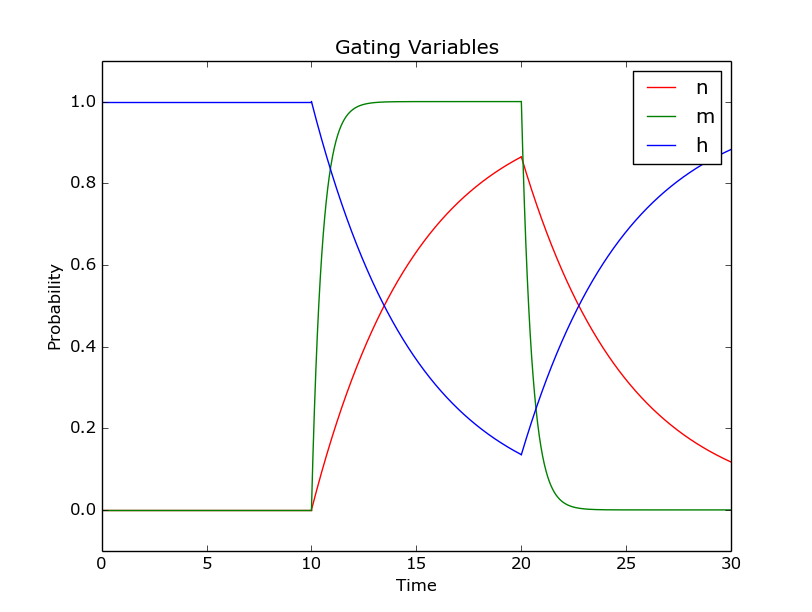
\includegraphics[scale=0.5]{gv.png}

For the conductances, I used the maximal sodium and potassium
conductance determined by Hodgkin and Huxley, $\bar g_{Na} = 120$, and
$\bar g_K = 36$. This gave the following functions

\[g_{Na}(t) = \bar g_{Na}m^3h = 120m^3h\]
\[g_K(t) = \bar g_Kn^4 = 36n^4\]

The plots for the above functions are shown below.

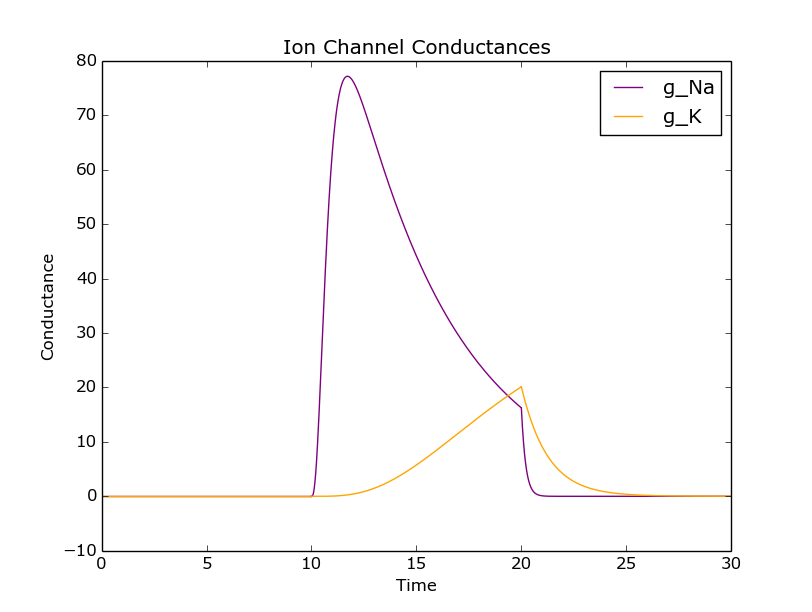
\includegraphics[scale=0.5]{con.png}

\subsubsection{(c)}\label{c}

Finally we combine all of the above information to define the ionic
currents.

\[I_{ion}(t) = g_{ion}(t)(V-V_{ion})\]

Over each interval, $(V-V_{ion})$ is different and the gating variable
equations change through the three equations outlined above. Instead of
defining all 6 equations here we will just show the plot of the behavior
over each interval.

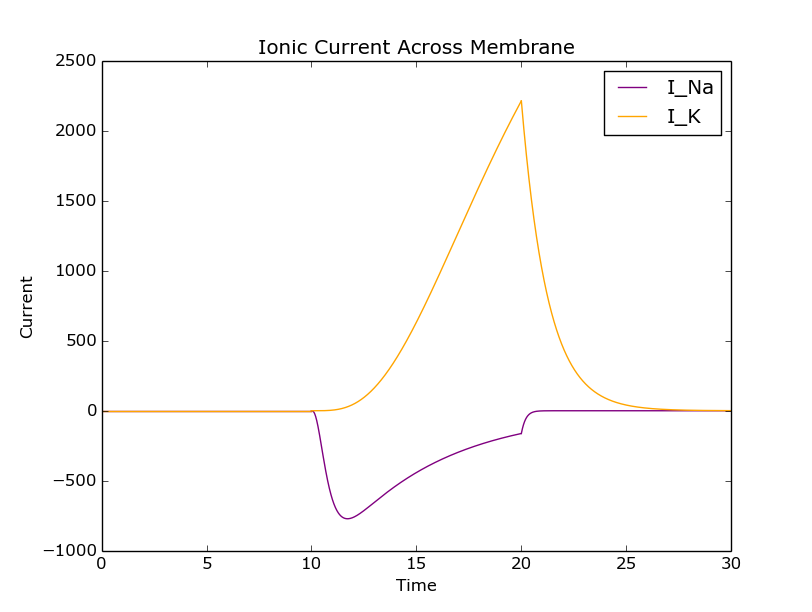
\includegraphics[scale=0.5]{cur.png}

    % Make sure that atleast 4 lines are below the HR
    \needspace{4\baselineskip}

    %
        %\vspace{6pt}
    %\makebox[0.1\linewidth]{\smaller\hfill\tt\color{nbframe-in-prompt}In\hspace{4pt}{[}{]}:\hspace{4pt}}\\*
    %\vspace{-2.65\baselineskip}
    %\begin{ColorVerbatim}
    %\vspace{-0.7\baselineskip}
    %\begin{Verbatim}[commandchars=\\\{\}]
    %
    %\end{Verbatim}
    %
    %
    %\vspace{0.3\baselineskip}
    %
    %\end{ColorVerbatim}
    

        

        \renewcommand{\indexname}{Index}
        \printindex

    % End of document
    \end{document}


